\documentclass[
]{beamer}

\usepackage[czech]{babel}
\usepackage[utf8]{inputenc}
\usepackage[T1]{fontenc}
\usepackage{csquotes}
\usepackage{expl3,biblatex}
\usepackage{hyperref}
\usepackage{booktabs}
\usetheme[
  workplace=fi,
]{MU}

\hypersetup{colorlinks,linkcolor=blue,urlcolor=blue}

\title{Verzovací systém git \& GitHub}
\subtitle{Workshop Poznej FI 2024}
\author[Honza Horáček]{Honza Horáček}
\institute[FI MU]{Spolek přátel severské zvěře, Fakulta informatiky, Masarykova univerzita}
\date{17. 2. 2024}
%\subject{}
%\keywords{}
\begin{document}


\begin{frame}[plain]
\maketitle
\end{frame}


\begin{frame}{Letem světem Linuxem}
\begin{itemize}
	\item Login na tabuli, přihlaste se.
	\item Stáhněte si slidy, napoví vám příkazy: \\ \url{https://poznej.fi.muni.cz/git.pdf}
\end{itemize}
\end{frame}

\begin{frame}{Letem světem Linuxem}
\begin{enumerate}
	\item Budeme používat git v terminálu (wtf?!).
	\item Základy práce s terminálem: \\
	prompt, souborový systém, \texttt{ls}, \texttt{cd}, \texttt{Ctrl+C}, man.
	\pause
	\item Textové editory: \texttt{vim}, \texttt{nano}, ...
\end{enumerate}
\end{frame}


\begin{frame}

\includegraphics[width=\textwidth]{images/vim1.png}
\end{frame}


\begin{frame}
\centering

\includegraphics[height=\textheight]{images/vim2.jpg}
\end{frame}


\begin{frame}{Prvotní konfigurace gitu}
Ovládání: \\
\texttt{\$ git <command>} \\
\vspace{1em}

\texttt{\$ git config -{}-global user.name "Honza Horacek"} \\
\pause
Kontrola: \texttt{\$ git config user.name} \\
\pause
\texttt{\$ git config -{}-global user.email "me@apophis.cz"} \\
\texttt{\$ git config -{}-global core.editor vim} :)
\pause

\begin{block}{Pro zvídavé}
\texttt{\$ git config -{}-list} \\
\texttt{\$ git config -{}-help}

Různé úrovně konfigurace: \texttt{-{}-system}, \texttt{-{}-global}, \texttt{-{}-local}
\end{block}
\end{frame}


\begin{frame}{Repozitář}

Repozitář obsahuje verzovaný projekt. Má svou vlastní historii, svoje soubory.

\begin{block}{Repozitář pro tento workshop}
Repozitář s Pythoním programem, který provádí jednoduché textové \uv{šifrovací} operace.
\end{block}

\begin{enumerate}
	\item \texttt{\$ mkdir pficipher}
	\item \texttt{\$ git init}
	\item \texttt{\$ git status}
	\item Šablona kódu: \url{https://poznej.fi.muni.cz/cipher.py}
\end{enumerate}
\end{frame}


\begin{frame}{add, commit, log}
\begin{columns}[T]
\begin{column}{.48\textwidth}
\begin{enumerate}
	\item \texttt{\$ git status}
	\item \texttt{\$ git add cipher.py}
	\item \texttt{\$ git status}
	\item \texttt{\$ git commit}
	\item \texttt{\$ git log}
\end{enumerate}

\end{column}

\begin{column}{.48\textwidth}
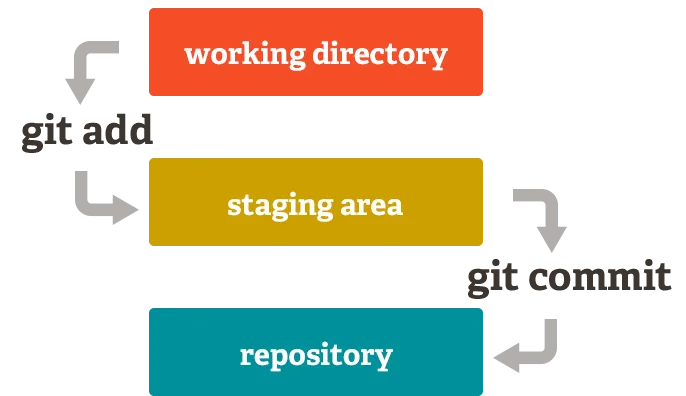
\includegraphics[width=\textwidth]{images/lifecycle.png}
\end{column}
\end{columns}

\pause

\begin{block}{Jak psát commit messages?}
\href{https://gist.github.com/robertpainsi/b632364184e70900af4ab688decf6f53}{Commit Message Guidelines} \\
\href{https://github.com/torvalds/linux}{Ukázka + proč vznikl git}
\end{block}

\begin{block}{Pro zvídavé}
\texttt{\$ git commit -m 'Add template of cipher.py.'} \\
\texttt{\$ git reset}
\end{block}
\end{frame}


\begin{frame}{Jdeme programovat!}
Implementujte nějakou funkci v \texttt{cipher.py}!

Zkuste si pracovat s příkazy:

\begin{itemize}
	\item \texttt{\$ git status}
	\item \texttt{\$ git add}
	\item \texttt{\$ git commit}
	\item \texttt{\$ git log}
	\item \texttt{\$ git reset}
	\item \texttt{\$ git commit -m <message>}
	\item \texttt{\$ git commit -a}
	\item \texttt{\$ git commit -{}-amend}
\end{itemize}

\begin{block}{Před použitím příkazu zjistěte, co dělají!}
\texttt{\$ git <command> -{}-help}
\end{block}

Vyrobte několik commitů.
\end{frame}


\begin{frame}{GitHub}
\centering
\url{https://github.com/} \vspace{1em} \\

\includegraphics[width=0.5\textwidth]{images/gitgithub.jpg}
\end{frame}


\begin{frame}{GitHub}
\begin{itemize}
	\item \href{https://github.com/horacekj}{Ukázka osobního účtu}
	\item \href{https://github.com/fi-ksi}{Ukázka organizace}
	\pause
	\item Vytvořte si účet.
	\item Založte si svůj prázdný repozitář \texttt{pficipher}.
	\item Projděte si nějaké repozitáře, proklikejte si webové rozhraní.
\end{itemize}
\end{frame}


\begin{frame}{Propojení gitu a GitHubu}
\begin{itemize}
	\item Git: distribuovaný systém s více možnými remotes.
	\item Základní workflow: jediný remote (alá GitHub).
	\item Komunikace s remote: více možností, my použijeme ssh (secure shell).
	\item \texttt{ssh-keygen} vytvoří pár klíčů.
	\begin{itemize}
		\item Privátní klíč si střežte jako oko v hlavě!
		\item Veřejný klíč (\texttt{.pub}) nahrajte do nastavení svého účtu na GitHub.
	\end{itemize}
\end{itemize}

\begin{block}{Pro zvídavé}
\href{https://linuxize.com/post/using-the-ssh-config-file/}{Soubor \texttt{.ssh/config}} umožňuje definovat,
pro jaké hosty se mají používat jaké ssh parametry (uživatelské jméno, klíč, ...).
\end{block}
\end{frame}


\begin{frame}{pull, push}
\texttt{\$ git remote add origin git@github.com:<user>/<repo>.git} \\
\texttt{\$ git push -u origin main} \\

\begin{itemize}
	\item \texttt{\$ git pull} – načte commity z remote
	\item \texttt{\$ git push} – odešle commity na remote
\end{itemize}

\begin{block}{Projekt}
\url{https://poznej.fi.muni.cz/test.py} \\
Vyzkoušejte si push \& pull. Zkuste udělat úpravu souboru přímo na GitHubu.
\end{block}
\end{frame}


\begin{frame}{Co když chci přepsat commit?}
\begin{itemize}
	\item Např. \texttt{push}, pak \texttt{commit -{}-amend}, pak \texttt{push}.
	\pause
	\item Velký problém – git hlídá kontinuitu historie.
	\item Řešení: primárně prevence, obecně pokročilejší téma.
\end{itemize}
\end{frame}


\begin{frame}{Spolupráce}
\begin{itemize}
	\item Udělte svému sousedovi přístup do repozitáře.
	\item Soused si váš repozitář stáhne k sobě do samostatného adresáře: \texttt{\$ git clone <remoteurl>}.
	\item Budete mít na počítači 2 podobné repozitáře, nesplěťte se!
	\item Zkuste pracovat v repozitáři souseda.
	\item Zkuste oba pracovat na stejném repozitáři.
	\begin{enumerate}
		\item Každý na jiném souboru.
		\item Oba na stejném souboru.
		\item Oba na stejném místě ve stejném souboru.
	\end{enumerate}
\end{itemize}
\end{frame}


\begin{frame}{Workflow, pull requesty, issues}
\begin{itemize}
	\item Typické workflow většího projektu: větve (\textit{branch}): \\
	\texttt{main}, \texttt{dev}, \texttt{feature<x>}.
	\item Feature pull request do dev. Dev release do main (dělá správce projektu).
	\item Vše je v jediném repozitáři.
\end{itemize}

\begin{figure}
	\centering
	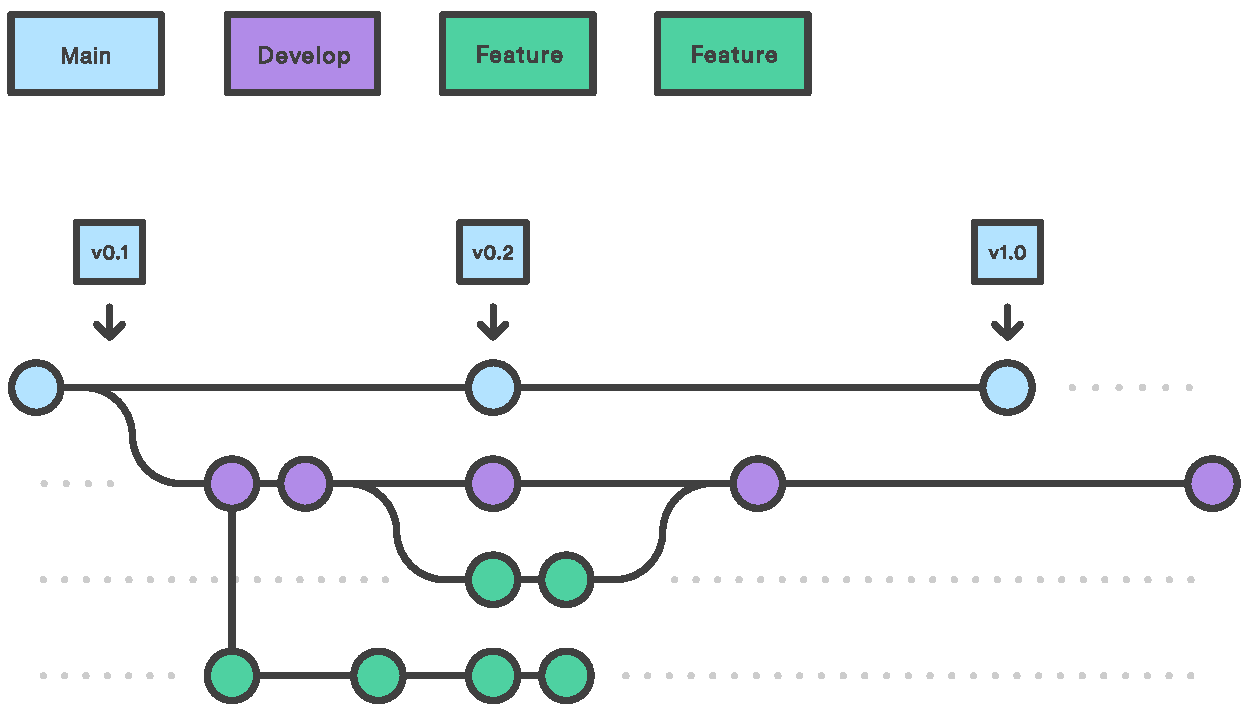
\includegraphics[width=0.6\textwidth]{images/features.pdf}
\end{figure}
\end{frame}


\begin{frame}{Větve}
\texttt{\$ git branch caesar} – vytvoří novou větev \\
\texttt{\$ git push -u origin caesar} – push nové větve (stačí poprvé) \\
\texttt{\$ git switch <branch>} – přepne stav souborů na HEAD větve <branch>

\begin{block}{Pro zvídavé}
\href{https://git-scm.com/book/en/v2/Git-Branching-Branches-in-a-Nutshell}{Branches in a Nutshell}
\end{block}

\begin{alertblock}{Úkol}
\begin{enumerate}
	\item Vytvořte feature kolegovi (použijte větev).
	\item Otevřte pull request.
	\item Kolega pull request přijme.
\end{enumerate}
\end{alertblock}
\end{frame}


\begin{frame}{Co stojí za vyzkoušení}
GitHub:
\begin{itemize}
	\item Issues a propojení s commit messages.
	\item Markdown – \texttt{README.md}.
	\item Releases a distribuce binárních souborů.
\end{itemize}

Git:
\begin{itemize}
	\item \texttt{.gitignore}
	\item \texttt{\$ git show}
	\item \texttt{\$ git diff}
	\item \texttt{\$ git tag}
\end{itemize}
\end{frame}


\begin{frame}{Slovo závěrem}
\begin{block}{Co dělat, když jsem si rozbil repozitář?}
Odpověď: nastudujte si \href{https://git-scm.com/doc}{dokumentaci gitu}, je
přehledná a detailní. Pak budete vědět, jak se dostat z prakticky libovolného stavu.
\end{block}

Co se hodí vědět:

\begin{itemize}
	\item git se obecně snaží nikdy nesmazat rozdělanou práci.
	\begin{itemize}
		\item Výjimka: použití přepínače \texttt{-{}-hard}. Pozor na něj!
	\end{itemize}
	\item \texttt{\$ git push -{}-force} často víc problémů způsobí než vyřeší.
	Pozor na něj!
\end{itemize}
\end{frame}

\end{document}
